\documentclass[twocolumn]{scrartcl}
\usepackage[cm]{fullpage}
\usepackage{hyperref}
\usepackage{graphicx}
\usepackage[backend=biber]{biblatex}
\addbibresource{report.bib}

\title{Classification of Wine Quality}
% Do NOT write your names here!
\author{Anonymous Authors}
\begin{document}
\maketitle

\section{Introduction}

The following report outlines our attempts to use common classification
algorithms to predict the wine quality depending on the given features.
We use a data set from the UCI Machine Learning Repository
\footnote{\url{http://archive.ics.uci.edu/ml/datasets/Wine+Quality}} \parencite{data}.

\subsection{Data Description}

The data set contains of 4898 data points, each of them described by 11 features
and an integer quality label ranging from 3 to 9.
Note that the distribution of the quality is unbalanced:
More than 90\% of the data points are assigned to a quality between 5 and 7 (Figure \ref{fig:unbal}).

\begin{figure}[h]
    \centering
    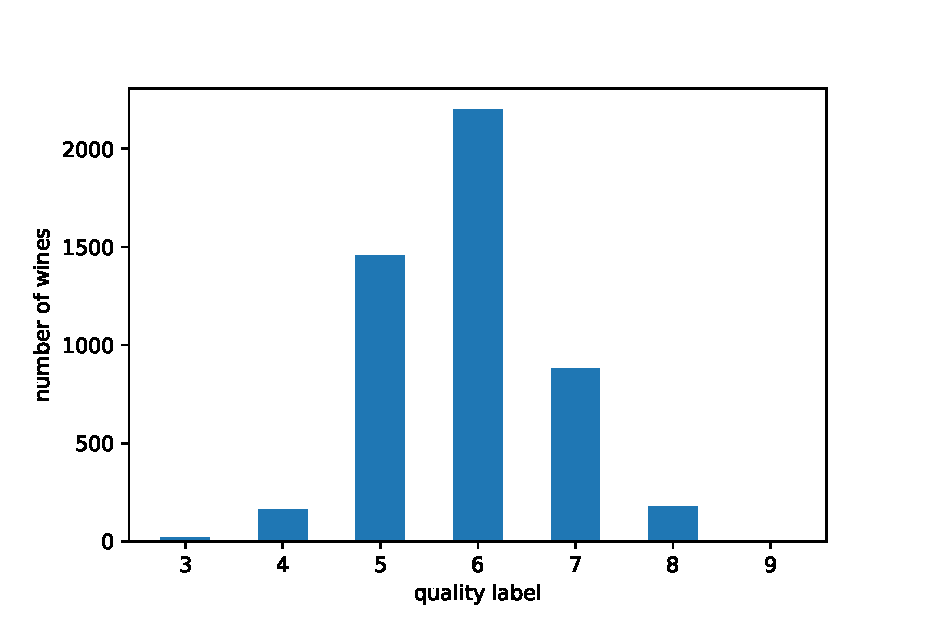
\includegraphics[width=\linewidth]{images/unbalanced.eps}
    \caption{distribution of quality}
    \label{fig:unbal}
\end{figure}

\subsection{Data preprocessing}

To simplify our problem we assigned new class labels 0, 1 and 2. We assign class 0 (bad) to wines ranging in qualities 3-5,
class 1 (medium) to wines labeled with quality 6 and class 2 (good) to wines with quality greater than 6.
We further decided to use classification instead of regression.
Though, it should be noted that we also examine algorithms (e.g. ridge classifier) that use regression to classify the data points
and using regression should therefore yield similar results in our case.
This doesn't come as a surprise, considering that the classes can obviously be linearly ordered.

%not yet decided which to use
\section{Ridge Classification}
\subsection{Description}
\subsection{Cross-Validation}
\subsection{Results}

\section{Multi Layer Perceptron (MLP)}
\subsection{Description}
MLP is a supervised learning algorithm and is a function approximator that can be used for classification and regression. We have used the MLPClassifier function (rather than MLPRegressor although both could be used on our  chosen data set) from scikit-learn's Neural Network library.

\subsection{Cross-Validation}
\subsection{Results}

\section{Random Forest Classification}
\subsection{Description}
Random Forest Classification is also a supervised learning algorithm that is widely used for solving classification and regression problems. The idea behind this method is to increase the classification accuracy (a.k.a aim for lower variance) by using bootstrap aggregating (or bagging) algorithms. Generally speaking, the gross idea behind Random Forest Classification is to use the bagging method to split up a decision tree into two different trees. When one does that enough times, there is a large amount of trees (hence the name- "forest) which gives the possibility to gather more information for analysis and therefore better accuracy. \footnote{\url{https://towardsdatascience.com/the-random-forest-algorithm-d457d499ffcd}}.
In this project we used the RandomForestClassifier algorithm from the Scikit-learn library.

\subsection{Cross-Validation}
\subsection{Results}

\section{Gaussian Process Classification}
\subsection{Description}
\subsection{Cross-Validation}
\subsection{Results}

\section{Comparison}
\section{Conclusion}

\printbibliography


\end{document}
